\documentclass[a4paper, 11pt]{article}

\usepackage{bm}  
\usepackage{float}
\usepackage{pdfsync}  
\usepackage{textcomp}
\usepackage{graphicx} 
\usepackage{fancyhdr}
\usepackage{memhfixc} 
\usepackage{etoolbox}
\usepackage{indentfirst}
\usepackage[utf8]{inputenc}
\usepackage{amsmath,amssymb}  
\usepackage[pdftex,bookmarks,colorlinks,breaklinks]{hyperref}  
\usepackage[top=3cm, bottom=3cm, left = 2cm, right = 2cm]{geometry} 
\usepackage[linesnumbered,ruled,vlined]{algorithm2e}

\AtBeginEnvironment{abstract}{\setlength{\parindent}{0pt}}

\geometry{a4paper} 
\hypersetup{linkcolor=black,citecolor=black,filecolor=black,urlcolor=black}

\title{Network Science Project \\ \textbf{Finding K-Cores of Large Graphs}}
\author{Guilherme Gonçalves \and João Silveira \and Manuel Brito}
\date{\today}

\begin{document}

\maketitle

\clearpage
\tableofcontents
\clearpage

\section{Introduction}
\label{sec:Introduction}

In the realm of network science and graph theory, the identification of cohesive substructures within complex networks is a fundamental task with far-reaching implications. One such critical concept is the k-core of a graph, a mathematical construct that characterizes the inherent structure and resilience of a network. K-cores offer valuable insights into the core-periphery organization of networks and have applications in various fields, including social network analysis, biology, transportation systems, and more.

The k-core of a graph represents a maximal subgraph where every vertex is connected to at least k other vertices within the subgraph. This concept is essential for understanding the robustness and functionality of real-world networks. As the value of k increases, the resulting k-core becomes progressively denser, unveiling the inner layers of a network's connectivity.

The process of identifying k-cores is not a trivial one, and researchers have developed multiple algorithms to efficiently compute them. These algorithms serve as the cornerstone for uncovering the intricate hierarchical structure within networks and have significant implications for various network-related applications.

This report embarks on a comparative study of two distinct algorithms for finding k-cores within a given graph. Our primary objective is to explore and evaluate the strengths and weaknesses of these algorithms in terms of computational efficiency, accuracy, and scalability. By doing so, we aim to provide valuable insights into the selection of an appropriate algorithm based on specific network characteristics and research objectives.

The two algorithms under consideration, which will be thoroughly analyzed and compared in this report, are the \textit{Degree Pruning Algorithm} and an algorithm that uses \textit{DFS} to solve the problem. Both algorithms have gained recognition in the field of network science and have shown promise in identifying k-cores effectively. However, they employ different strategies and heuristics, which may lead to variations in their performance under different network scenarios.

In the subsequent sections of this report, we will delve into the theoretical foundations of k-cores, provide an in-depth explanation of the chosen algorithms, present our experimental methodology, and report the findings of our comparative analysis. By the conclusion of this study, readers will have a comprehensive understanding of the intricacies involved in identifying k-cores and will be equipped with insights to make informed decisions about the choice of algorithm for their specific network analysis tasks.


\section{Algorithms Overview}
\label{Algorithms}

\subsection{Degree Pruning Algorithm}

\subsubsection{Overview}

The degree-running algorithm is a widely used and efficient method for discovering k-cores within a graph. It accomplishes this by utilizing the concept of "vertex degree," which denotes the number of edges connected to a vertex. This algorithm progressively removes vertices and edges with degrees less than the desired k, ultimately revealing the k-core structure of the graph. It is especially effective in scenarios where the graph is sparse or moderately dense, making it a valuable tool for various network analysis tasks. In summary, the algorithm leverages vertex degrees to iteratively prune the graph until the desired k-core is achieved, providing insights into network organization.

Initially, the algorithm calculates the degree of every node and enqueues nodes with degrees less than $k$. Subsequently, it dequeues nodes from the queue one at a time, removes them from the graph, and decreases the degrees of their neighbors. If, at any stage, a node's degree falls below $k$, it is also placed in the queue for removal. Ultimately, only the k-core of the graph remains intact after this process. A pseudo-code for the algorithm in question can be found in algorithm \ref{algo:degree-pruning}

\begin{algorithm}[htb]
    \label{algo:degree-pruning}
    \caption{Degree-Pruning Algorithm}
    
    \SetKwFunction{Kcores}{KCores}
    \SetKwProg{Fn}{Function}{:}{}
    \Fn{\Kcores{$g$, $k$}}{
        $q \leftarrow$ empty queue of size $|V|$\;
        $degree \leftarrow$ array of size $|V|$ (initialized with degrees of vertices in $g$)\;
        \For{$i \leftarrow 0$ \KwTo $|V| - 1$}{
            $d \leftarrow$ degree of vertex $i$ in $g$\;
            \If{$d < k$}{
                $q$.enqueue($i$)\;
            }
            $degree[i] \leftarrow d$\;
        }
        \While{$q$ is not empty}{
            $u \leftarrow q$.dequeue()\;
            \ForEach{neighbor $v$ of $u$ in $g$}{
                \If{$degree[v] \geq k$}{
                    $degree[v] \leftarrow degree[v] - 1$\;
                    \If{$degree[v] < k$}{
                        $q$.enqueue($v$)\;
                    }
                }
            }
            Remove vertex $u$ from $g$\;
        }
        $cores \leftarrow$ empty list\;
        \For{$i \leftarrow 0$ \KwTo $|V| - 1$}{
            \If{degree of vertex $i$ in $g \geq k$}{
                $cores$.append($i$)\;
            }
        }
        \KwRet $cores$\;
    }
\end{algorithm}

\subsubsection{Complexity Analysis}

Computing the space complexity of this algorithm is trivial, since it uses a vector of size $|G|$ and a queue that can have atmost the same size. Thus, we can say that the space complexity is $O(|G|)$, meaning that the space complexity is $O(V)$.

The time complexity will depend on two factors: the dequeuing (which has a time complexity of $O(V)$, since if there is no k-core all nodes will end up in the queue) loop and visiting the neighbours (which has a time complexity, in the worst case, equal to the number of edges, $O(E)$). Therefore, the final complexity is $O(V + E)$. Not that the number $k$ influences the complexity, because nodes are added to the queue, and, consequently more neighbours are visited, based on the relationship between their degree and $k$

\subsection{Depth-First Search Based Algorithm}

\subsubsection{Overview}

The \textbf{K-Cores Algorithm} aims to identify the subgraph formed by vertices with degrees greater than or equal to a specified threshold \(k\). Utilizing a Depth-First Search (DFS) strategy, the algorithm efficiently explores the graph structure to identify the K-Cores.

\begin{enumerate}
    \item \textbf{Initialization:} The algorithm initializes a \texttt{visited} array to keep track of visited vertices and a \texttt{degree} array to store the degrees of vertices in the graph \(g\). The DFS traversal begins with a vertex having the minimum degree.
    
    \item \textbf{Depth-First Search (DFS):} The algorithm performs a DFS traversal starting from the initial vertex. During DFS, it decrements the degrees of neighbors, marking them as visited if their degrees drop below \(k\). Disconnected components are handled by subsequent DFS passes.
    
    \item \textbf{Degree Adjustment:} After DFS, the algorithm adjusts the degrees of vertices based on their neighbors with degrees greater than or equal to \(k\).
    
    \item \textbf{Identifying K-Cores:} Vertices with degrees greater than or equal to \(k\) are collected into the \texttt{cores} list, forming the K-Cores subgraph.
\end{enumerate}

\begin{itemize}
    \item \textbf{DFS Traversal:} The algorithm explores the graph using DFS, adjusting degrees and marking vertices as visited based on their degrees and neighbors' degrees.
    
    \item \textbf{Degree Adjustment:} Degrees of vertices are recalculated based on their neighbors with degrees greater than or equal to \(k\).
    
    \item \textbf{Subgraph Construction:} Vertices with degrees above or equal to \(k\) are added to the \texttt{cores} list, forming the K-Cores subgraph of the input graph.
\end{itemize}

\begin{algorithm}[H]
    \label{algo:dfs-based}
    \caption{Depth-First Search Based Algorithm}

    \SetKwFunction{DFS}{DFS}
    \SetKwFunction{FindKCoresDFS}{findKCoresDFS}
    \SetKwProg{Fn}{Function}{:}{}
    \Fn{\DFS{$u$, $g$, $visited$, $degree$, $k$}}{
        stack $\leftarrow$ empty stack\;
        stack.push($u$)\;
        visited[$u$] $\leftarrow$ true\;

        \While{stack is not empty}{
            $v \leftarrow$ stack.pop()\;
            \If{$degree[v] < k$}{
                \ForEach{neighbor $w$ of $v$ in $g$}{
                    \If{not visited[$w$]}{
                        stack.push($w$)\;
                        visited[$w$] $\leftarrow$ true\;
                        $degree[w] \leftarrow degree[w] - 1$\;
                    }
                }
            }
            \Else{
                \ForEach{neighbor $w$ of $v$ in $g$}{
                    \If{not visited[$w$]}{
                        stack.push($w$)\;
                        visited[$w$] $\leftarrow$ true\;
                    }
                }
            }
        }
    }
    \Fn{\FindKCoresDFS{$g$, $k$}}{
        visited $\leftarrow$ array of size $|V|$ (initialized to false)\;
        degree $\leftarrow$ array of size $|V|$ (initialized with degrees of vertices in $g$)\;
        startVertex $\leftarrow$ vertex with minimum degree in $g$\;

        \DFS{startVertex, $g$, visited, degree, $k$}\;

        \ForEach{vertex $v$ in $g$}{
            \If{not visited[$v$]}{
                \DFS{$v$, $g$, visited, degree, $k$}\;
            }
        }

        \ForEach{vertex $v$ in $g$}{
            \If{$degree[v] \geq k$}{
                count $\leftarrow$ 0\;
                \ForEach{neighbor $w$ of $v$ in $g$}{
                    \If{$degree[w] \geq k$}{
                        count $\leftarrow$ count + 1\;
                    }
                }
                $degree[v] \leftarrow$ count\;
            }
        }

        cores $\leftarrow$ empty list\;
        \ForEach{vertex $v$ in $g$}{
            \If{$degree[v] \geq k$}{
                cores.append($v$)\;
            }
        }

        \KwRet cores\;
    }
\end{algorithm}

\subsubsection{Complexity Analysis}

\begin{itemize}
    \item \textbf{Time Complexity:} The algorithm's time complexity is determined by the DFS traversal and is generally linear in the number of edges and vertices.
    
    \item \textbf{Space Complexity:} The algorithm's space complexity primarily depends on the storage of the \texttt{visited} and \texttt{degree} arrays, making it linear in the number of vertices.
\end{itemize}

\section{Evaluation}
\label{Evaluation}

In order to evaluate the performance of both alorithms, we implemented them in C++ \footnote{\url{https://github.com/jsilll/crc}} using the Boost Graph Library's (BGL) \footnote{\url{https://www.boost.org/doc/libs/1_82_0/libs/graph/doc/index.html}} graph data structure. This allowed us to easily generate random graph instances and to use the BGL's built-in functions to visualize the graphs and the k-cores. Moreover, having the both algorithms implemented in the same language and using the same graph data structure allowed us to compare them in a fair way.

To benchmark the algorithms, we used various graphs from the Stanford Network Analysis Project (SNAP) \footnote{\url{https://snap.stanford.edu/data/}}. We ran the algorithms for all the $k$ values between 1 and the maximum degree of the graph. The results are presented in figures \ref{fig:amazon}, \ref{fig:cit-patents}, \ref{fig:tech-as-skitter}, \ref{fig:web-google} and \ref{fig:wikitalk}.

All the benchmarks were run on a computer with an Intel Core i5-8250U CPU and 8GB of RAM. The operating system was Fedora 38. The compiler used was Clang 16.0.4. The compiler flags used were \texttt{-O3} and \texttt{-march=native}.

\begin{figure}[H]
    \centering
    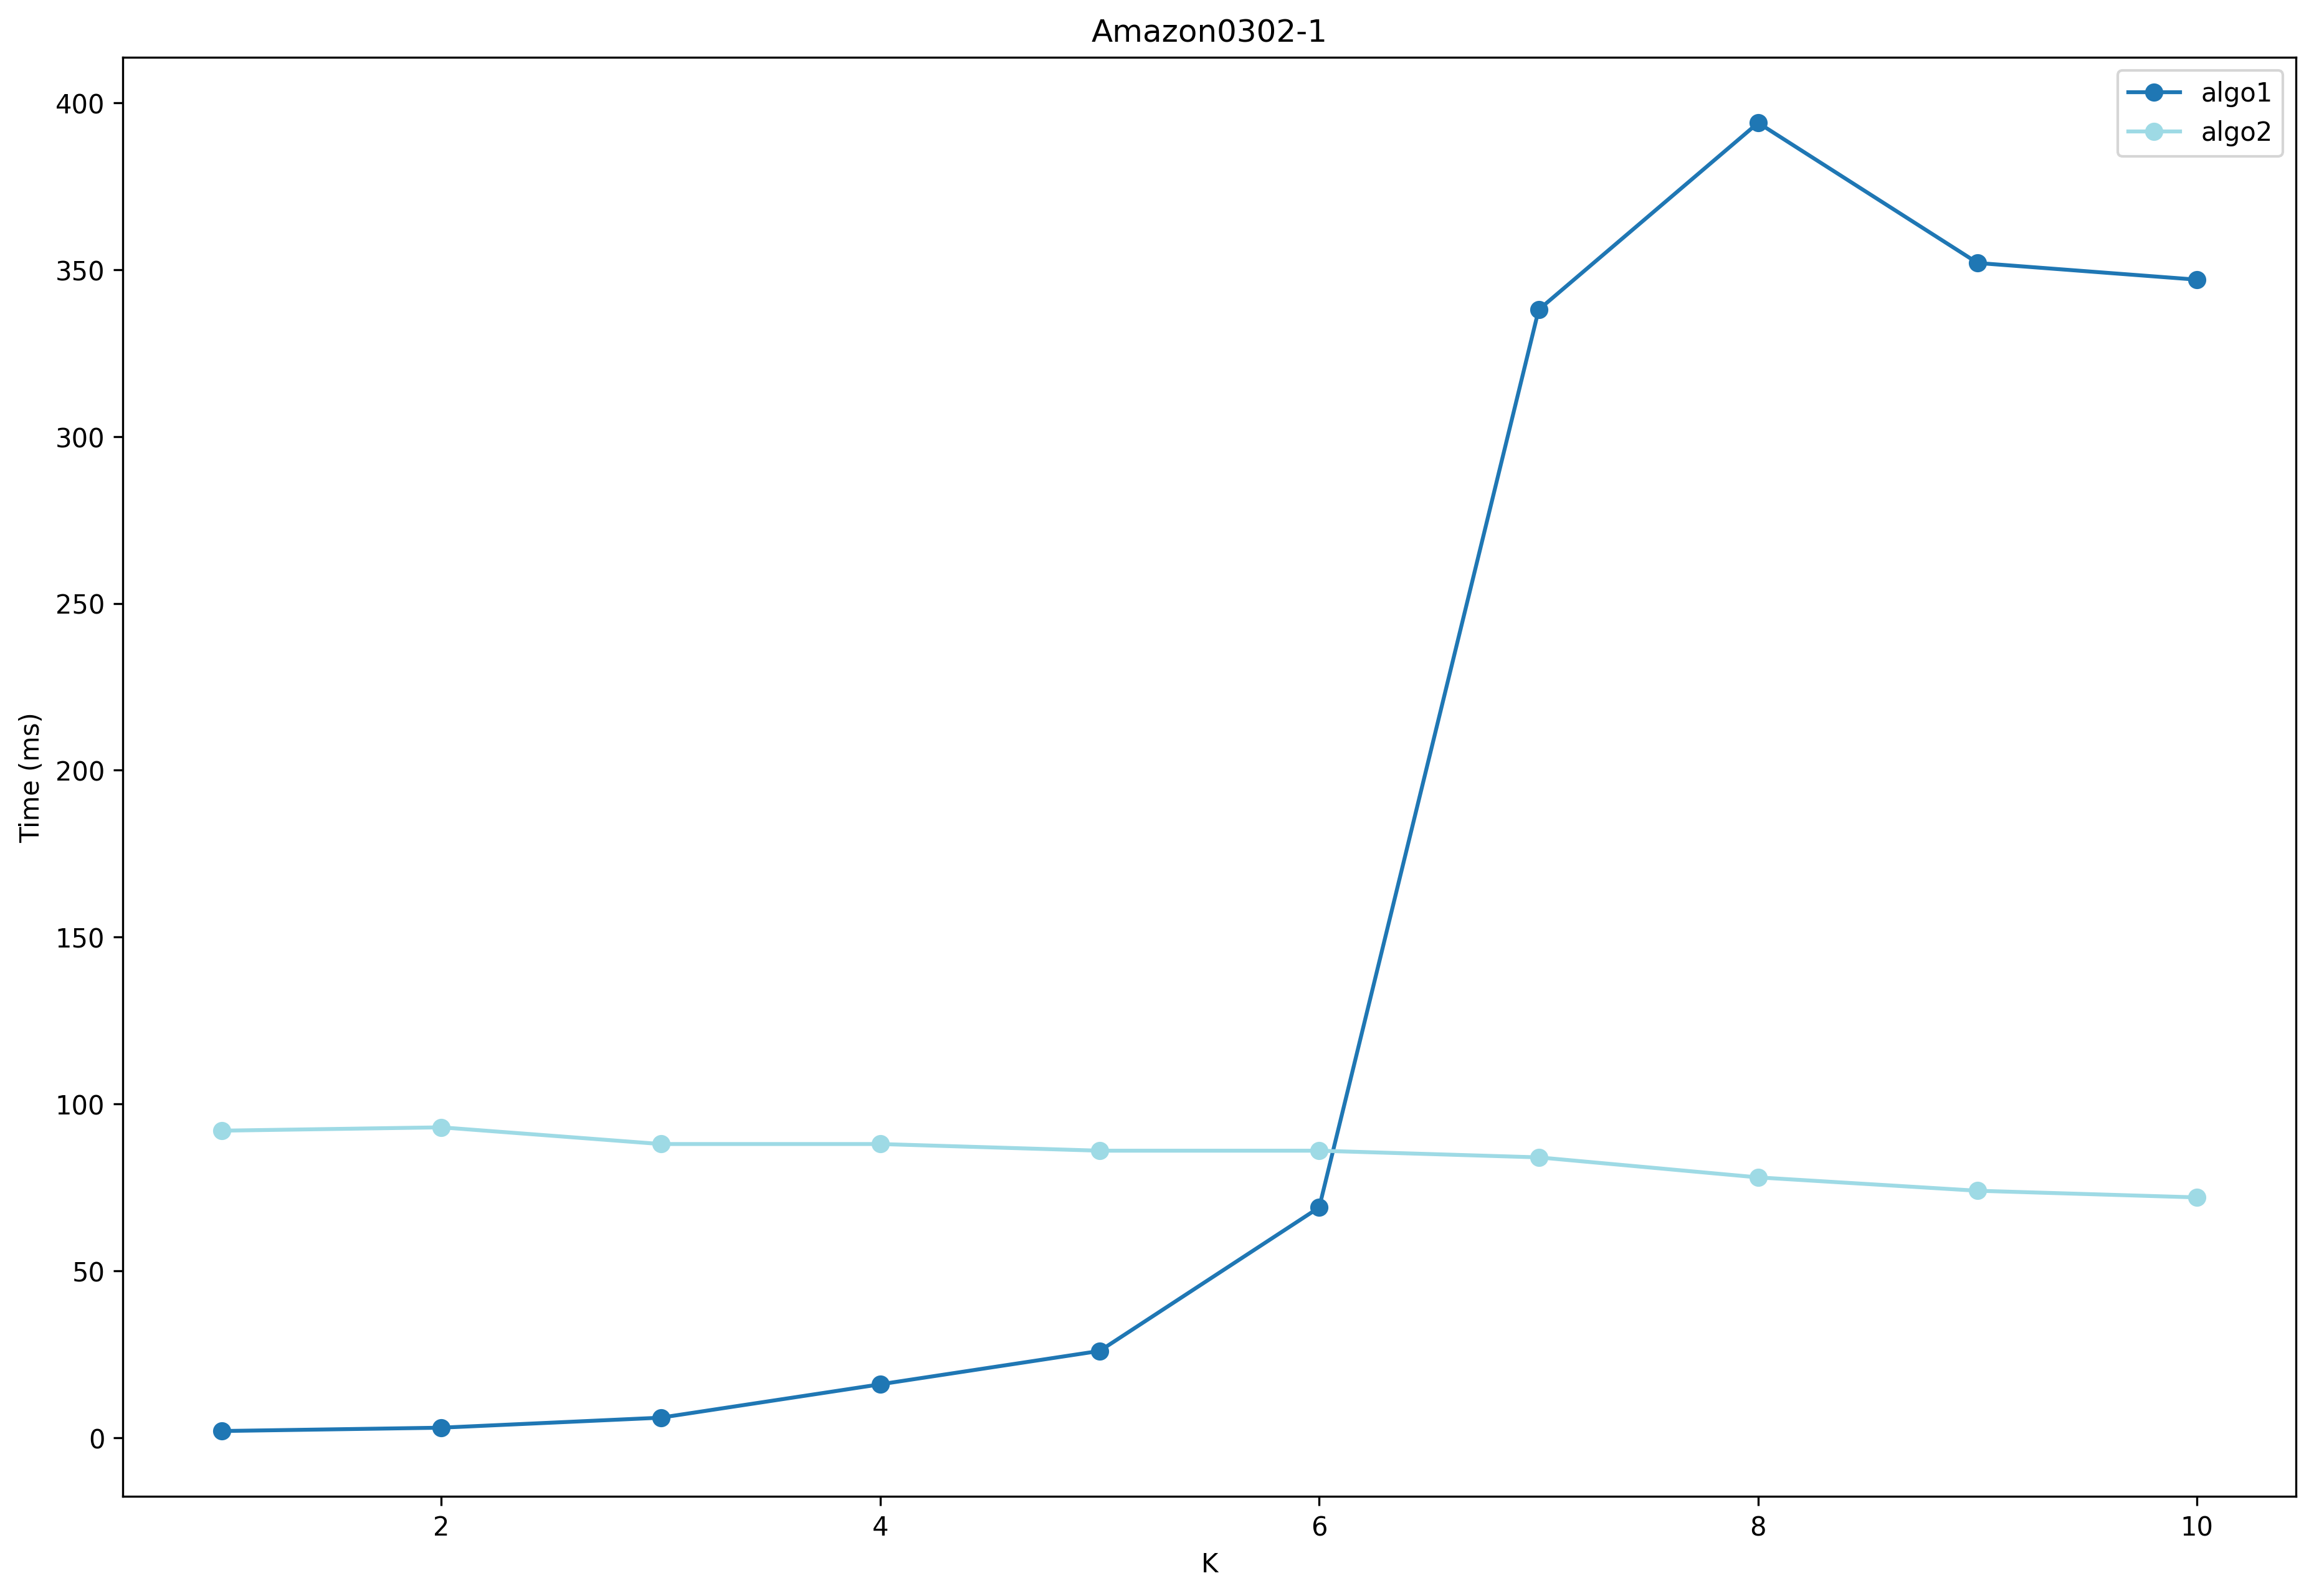
\includegraphics[width=0.6\textwidth]{Figures/Amazon0302-1.png}
    \caption{Amazon0302 benchmark times for both algorithms}
    \label{fig:amazon}
\end{figure}

\begin{figure}[H]
    \centering
    \includegraphics[width=0.6\textwidth]{Figures/cit-Patents.png}
    \caption{cit-Patents benchmark times for both algorithms}
    \label{fig:cit-patents}
\end{figure}

\begin{figure}[H]
    \centering
    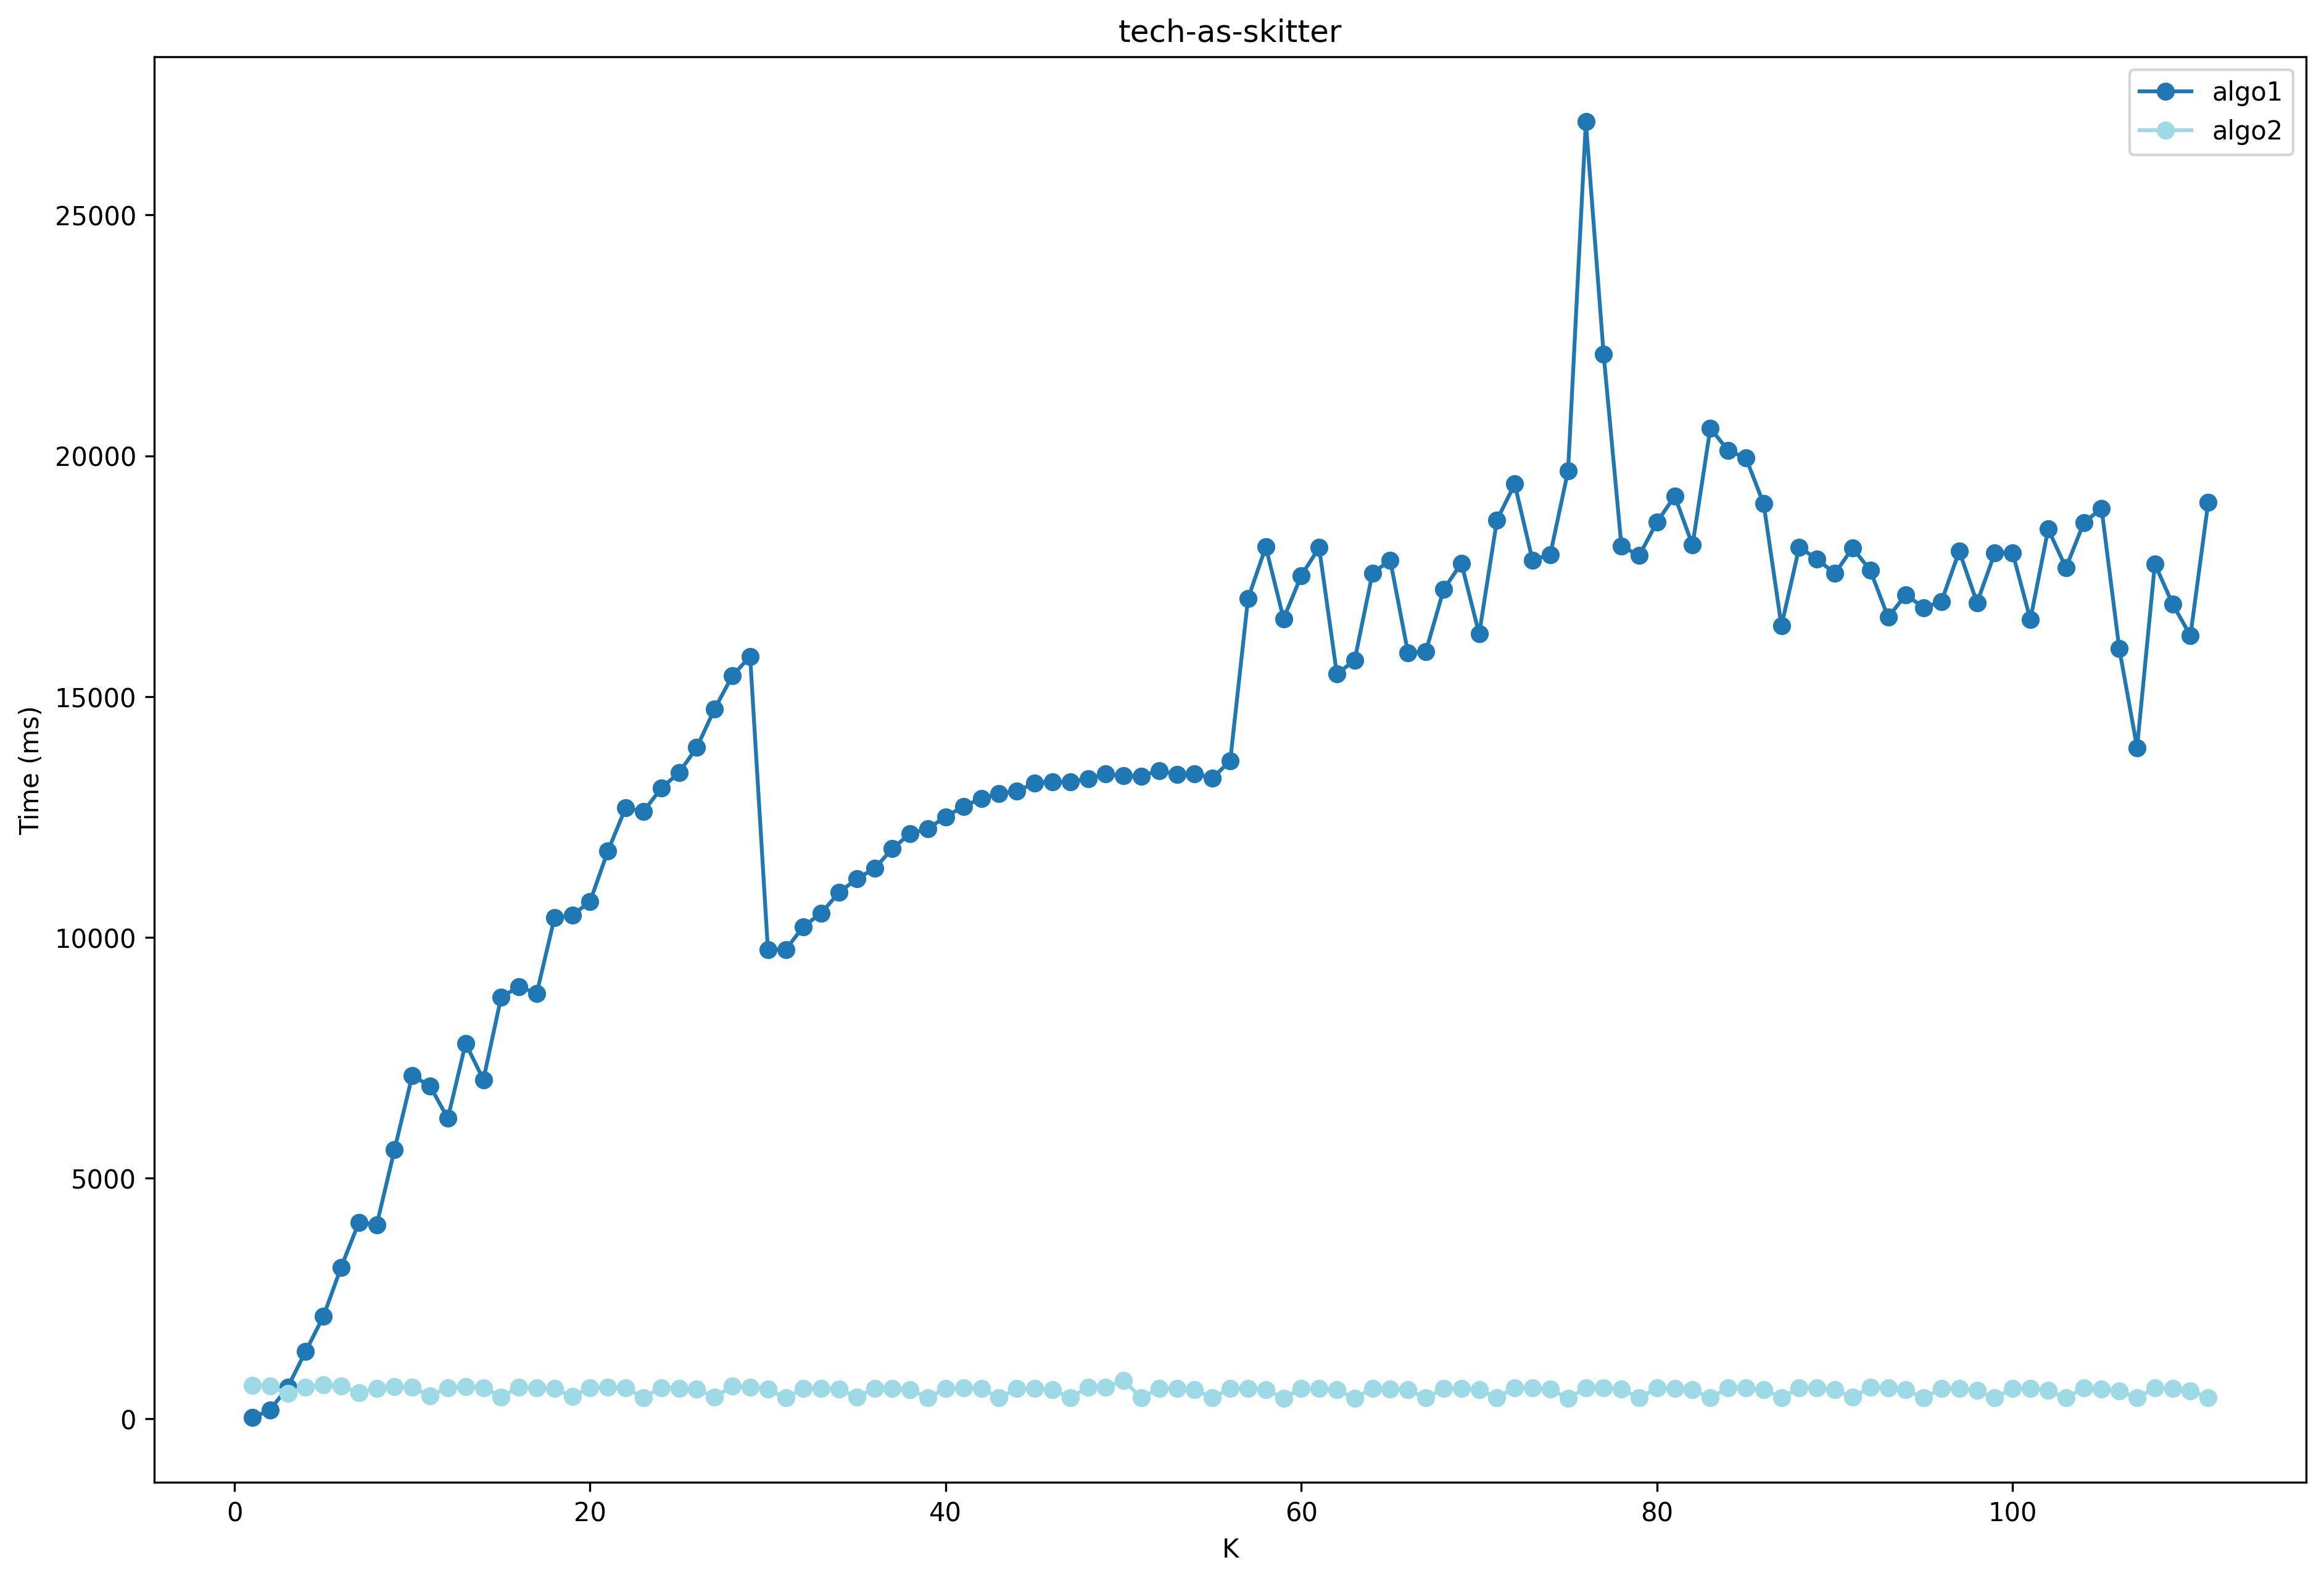
\includegraphics[width=0.6\textwidth]{Figures/tech-as-skitter.png}
    \caption{tech-as-skitter benchmark times for both algorithms}
    \label{fig:tech-as-skitter}
\end{figure}

\begin{figure}[H]
    \centering
    \includegraphics[width=0.6\textwidth]{Figures/web-Google.png}
    \caption{web-Google benchmark times for both algorithms}
    \label{fig:web-google}
\end{figure}

\begin{figure}[H]
    \centering
    \includegraphics[width=0.6\textwidth]{Figures/WikiTalk.png}
    \caption{WikiTalk benchmark times for both algorithms}
    \label{fig:wikitalk}
\end{figure} 

The results show that the depth-first search based algorithm is consistently much faster than the degree-pruning algorithm. This is possibly due to the removal of vertices and edges in the degree-pruning algorithm, which is a costly operation. The depth-first search based algorithm, on the other hand, only needs to keep track of the degrees of the vertices and the visited vertices, which is a much simpler task.

\section{Future Work}
TODO: Dizer que podemos explorar a possibilidade de usar MPI e OpenMP para paralelizar ambos os algoritmos.

\section{Conclusion}
\label{Conclusion}

The K-Cores Problem represents a powerful paradigm in graph theory and network analysis, offering nuanced insights into the intricate world of interconnected systems. By delving into cohesive substructures within networks, this concept has far-reaching implications across various domains.

In order to identify the K-Cores in a graph, we evaluated two algorithms on a set of benchmarks, the Degree Pruning algorithm and a Depth-First Search approach to the K-Cores problem. Due to, primarily, the queue's size and the duplication of nodes, the Degree Pruning Algorithm is way less efficient than its Depth-First Search counter part. However, these conclusions are limited by the set of benchmarks used.

Although there is more research to be made in this area, as mentioned in section \ref{FutureWork}, this study contributed to identifying the most efficient algorithms for solving the K-Cores problem. As networks continue to evolve and expand in complexity, the K-Cores Problem remains a cornerstone in understanding their underlying structures with applications in diverse fields, making it an indispensable asset in the toolkit of network analysts and researchers worldwide.


\clearpage
\bibliographystyle{abbrv}
\bibliography{Bibliography}
\end{document}